There are $N$ small towns in Kazakhstan, numbered from $0$ through $N - 1$. There is also an unknown number of large cities. The small towns and large cities of Kazakhstan are jointly called \textit{settlements}.

All the settlements of Kazakhstan are connected by a single network of bidirectional highways. Each highway connects two distinct settlements, and each pair of settlements is directly connected by at most one highway. For each pair of settlements $a$ and $b$ there is a unique way in which one can go from $a$ to $b$ using the highways, as long as no highway is used more than once.

It is known that each small town is directly connected to a single other settlement, and each large city is directly connected to three or more settlements.

The following figure shows a network of 11 small towns and 7 large cities. Small towns are depicted as circles and labeled by integers, large cities are depicted as squares and labeled by letters.

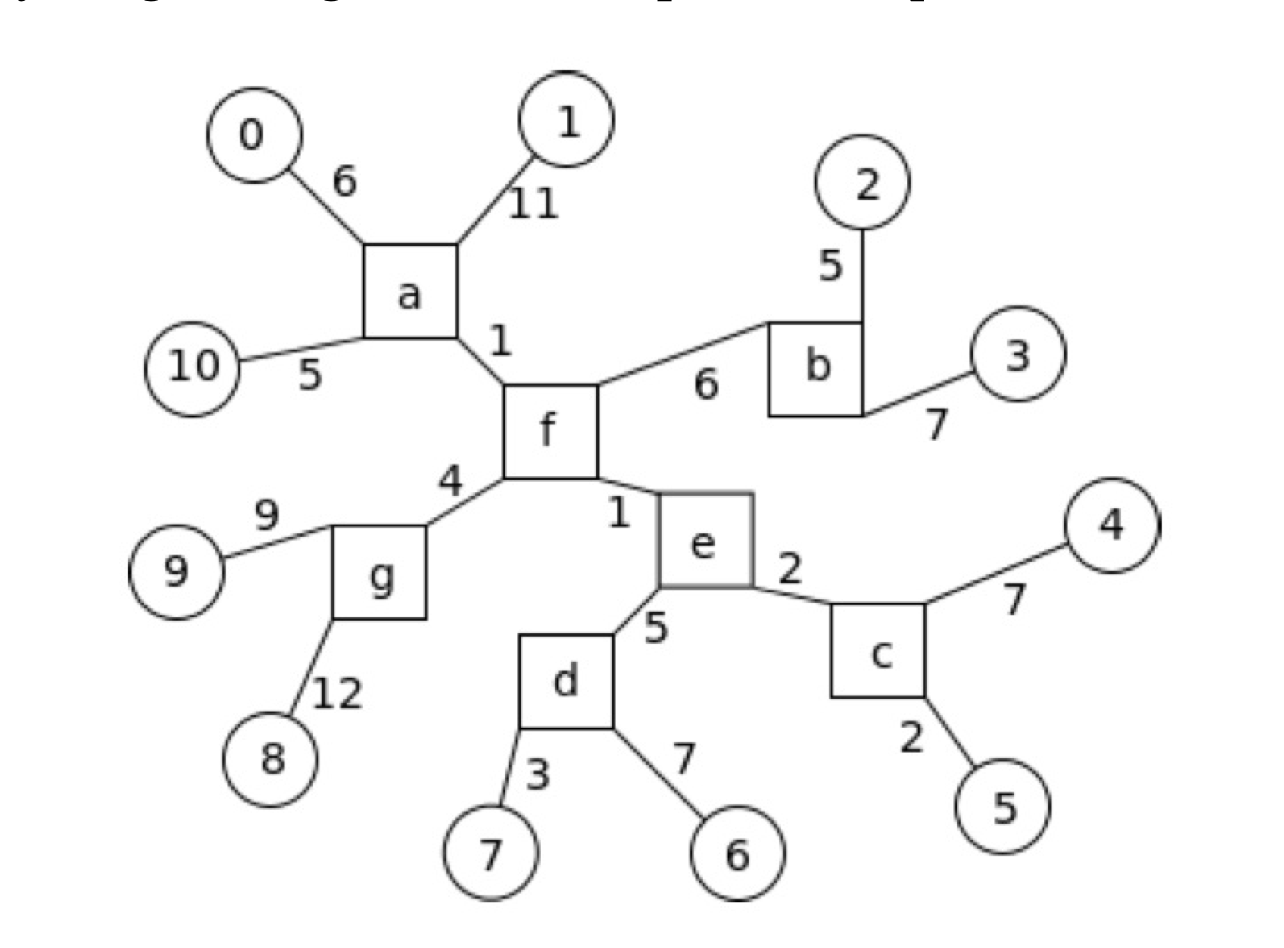
\includegraphics[scale=0.8]{towns.png}

Every highway has a positive integer length. The distance between two settlements is the minimum sum of the lengths of the highways one needs to travel in order to get from one settlement to the other.

For each large city $C$ we can measure the distance $r(C)$ to the small town that is the farthest away from that city. A large city $C$ is a hub if the distance $r(C)$ is the smallest among all large cities. The distance between a hub and a small town that is farthest away from the hub will be denoted by $R$. Thus, $R$ is the smallest of all values $r(C)$.

In the above example the farthest small town from city $a$ is town 8, and the distance between them is $r(a) = 1 + 4 + 12 = 17$. For city $g$ we also have $r(g) = 17$. (One of the small towns that are farthest away from $g$ is town 6.) The only hub in the above example is city $f$, with $r(f) = 16$. Hence, in the above example $R$ is 16.

Removing a hub divides the network into multiple connected pieces. A hub is \textit{balanced} if each of those pieces contains at most $\lfloor \frac{N}{2} \rfloor$ small towns. (We stress that we do not count the large cities.) Note that $\lfloor x \rfloor$ denotes the largest integer which is not greater than $x$.

In our example, city $f$ is a hub. If we remove city $f$, the network will break into four connected pieces. These four pieces consist of the following sets of small towns: {$0, 1, 10$}, {$2, 3$}, {$4,5,6,7$}, and {$8, 9$}. None of these pieces has more than  $\lfloor \frac{11}{2} \rfloor = 5$ small towns, hence city $f$ is a balanced hub.

\textbf{Task}

Initially, the only information you have about the network of settlements and highways is the number $N$ of small towns. You do not know the number of large cities. You also do not know anything about
the layout of highways in the country. You can only obtain new information by asking queries about distances between pairs of small towns.

Your task is to determine:
\begin{itemize}
\item In all subtasks: the distance $R$.
\item In subtasks $3$ to $6$: whether there is a balanced hub in the network.
\end{itemize}

You need to implement the function \texttt{hubDistance}. The grader will evaluate multiple test cases in a single run. The number of test cases per run is at most 40. For each test case the grader will call your
function \texttt{hubDistance} exactly once. Make sure that your function initializes all necessary variables every time it is called.

\begin{itemize}
\item \texttt{int hubDistance(int N, int sub)}
\begin{itemize}
\item $N$: the number of small towns.
\item $sub$: the subtask number (explained in the Scoring section).
\item If $sub$ is 1 or 2, the function can return either $R$ or $-R$.
\item if $sub$ is greater than 2, if there exists a balanced hub then the function must return $R$, otherwise it must return $-R$.
\end{itemize}
\end{itemize}

Your function \texttt{hubDistance} can obtain information about the network of highways by calling the grader function \texttt{getDistance(i, j)}. This function returns the distance between the small towns $i$ and $j$. Note that if $i$ and $j$ are equal, the function returns 0. It also returns 0 when the arguments are invalid.